\section{Differential Geometry}
\label{sec:differential_geometry}

We start this section by developing the necessary mathematical tools and concepts required to understand geometric inverse problems. This section just briefly introduces concepts from differential and riemannian geometry that are used throughout this paper.

\subsection{Intro to Manifolds} Let's begin by introducing the concept of a manifold.
\begin{definition}
  An \emph{$n$-dimension manifold}, $M$, is a topological space such that
  \begin{enumerate}
    \item $M$ is locally Euclidean, i.e., for every point $p \in M$, there exists an open neighborhood $U$ of $p$ and a homeomorphism $\phi : U \to V \subset \R^n$, where $V$ is an open subset of $\R^n$. We call the pair $(U, \phi)$ a \emph{chart} of $M$.
    \item $M$ is Hausdorff, i.e., for any two distinct points $p, q \in M$, there exist disjoint open neighborhoods $U_p$ and $U_q$ such that $p \in U_p$ and $q \in U_q$.
    \item $M$ is second countable, i.e., there exists a countable basis for the topology of $M$.
  \end{enumerate}
\end{definition}
We define an \textit{atlas} as the collection of all the charts along with their transition maps, $\mathcal{A} = \{(U_i, \phi_i)\}$. To go from one chart, $U_i$, to another chart, $U_j$, if $U_i \cap U_j \ne \emptyset$, we can use the transition maps:
\[%
  \phi_j \circ \phi_i^{-1} : \phi_i(U_i \cap U_j) \to \phi_j(U_i \cap U_j)
.\]%
But, throughout this paper, we only care about smooth manifolds, which are manifolds that are endowed with a smooth structure. Before doing so, we first need to define what a smooth map is.
\begin{figure}[h]
  \centering

  \begin{tikzpicture}

    % Functions i
    \path[->] (0.8, 0) edge [bend right] node[left, xshift=-2mm] {$\phi_i$} (-1, -2.9);
    \draw[white,fill=white] (0.06,-0.57) circle (.15cm);
    \path[->] (-0.7, -3.05) edge [bend right] node [right, yshift=-3mm] {$\phi^{-1}_i$} (1.093, -0.11);
    \draw[white, fill=white] (0.95,-1.2) circle (.15cm);

    % Functions j
    \path[->] (5.8, -2.8) edge [bend left] node[midway, xshift=-5mm, yshift=-3mm] {$\phi^{-1}_j$} (3.8, -0.35);
    \draw[white, fill=white] (4,-1.1) circle (.15cm);
    \path[->] (4.2, 0) edge [bend left] node[right, xshift=2mm] {$\phi_j$} (6.2, -2.8);
    \draw[white, fill=white] (4.54,-0.12) circle (.15cm);

    % Manifold
    \draw[smooth cycle, tension=0.4, fill=white, pattern color=brown, pattern=north west lines, opacity=0.7] plot coordinates{(2,2) (-0.5,0) (3,-2) (5,1)} node at (3,2.3) {$M$};

    % Subsets
    \draw[smooth cycle, pattern color=orange, pattern=crosshatch dots]
      plot coordinates {(1,0) (1.5, 1.2) (2.5,1.3) (2.6, 0.4)}
      node [label={[label distance=-0.3cm, xshift=-2cm, fill=white]:$U_i$}] {};
    \draw[smooth cycle, pattern color=blue, pattern=crosshatch dots]
      plot coordinates {(4, 0) (3.7, 0.8) (3.0, 1.2) (2.5, 1.2) (2.2, 0.8) (2.3, 0.5) (2.6, 0.3) (3.5, 0.0)}
      node [label={[label distance=-0.8cm, xshift=.75cm, yshift=1cm, fill=white]:$U_j$}] {};

    % First Axis
    \draw[thick, ->] (-3,-5) -- (0, -5) node [label=above:$\phi_i(U_i)$] {};
    \draw[thick, ->] (-3,-5) -- (-3, -2) node [label=right:$\R^m$] {};

    % Arrow from i to j
    \draw[->] (0, -3.85) -- node[midway, above]{$\psi_{ij} = \phi_j \circ \phi_i^{-1}$} (4.5, -3.85);

    % Second Axis
    \draw[thick, ->] (5, -5) -- (8, -5) node [label=above:$\phi_j(U_j)$] {};
    \draw[thick, ->] (5, -5) -- (5, -2) node [label=right:$\R^m$] {};

    % Sets in R^m
    \draw[white, pattern color=orange, pattern=crosshatch dots] (-0.67, -3.06) -- +(180:0.8) arc (180:270:0.8);
    \fill[even odd rule, white] [smooth cycle] plot coordinates{(-2, -4.5) (-2, -3.2) (-0.8, -3.2) (-0.8, -4.5)} (-0.67, -3.06) -- +(180:0.8) arc (180:270:0.8);
    \draw[smooth cycle] plot coordinates{(-2, -4.5) (-2, -3.2) (-0.8, -3.2) (-0.8, -4.5)};
    \draw (-1.45, -3.06) arc (180:270:0.8);

    \draw[white, pattern color=blue, pattern=crosshatch dots] (5.7, -3.06) -- +(-90:0.8) arc (-90:0:0.8);
    \fill[even odd rule, white] [smooth cycle] plot coordinates{(7, -4.5) (7, -3.2) (5.8, -3.2) (5.8, -4.5)} (5.7, -3.06) -- +(-90:0.8) arc (-90:0:0.8);
    \draw[smooth cycle] plot coordinates{(7, -4.5) (7, -3.2) (5.8, -3.2) (5.8, -4.5)};
    \draw (5.69, -3.85) arc (-90:0:0.8);

  \end{tikzpicture}

  \caption{Transition maps between charts on a manifold.}
  \label{fig:manifold_charts}
\end{figure}

\begin{definition}
  If $U$ and $V$ are open subsets of $\R^n$ and $\R^m$, then $F : U \to V$ is said to be \emph{smooth}\footnote{Some authors use ``smooth'' to denote infinitely differentiable ($C^\infty$), some use it to indicate just $k$-differentiable ($C^k$). I use it to denote $C^\infty$.} if each of $F$'s component functions are continuous and have continuous partial derivatives. In addition, if $F$ is bijective, then $F$ is called a \emph{diffeomorphism}.
\end{definition}
We can formally define a smooth manifold as follows.
\begin{definition}
  A \emph{$k$-differentiable manifold} is a manifold $M$ equipped with an atlas $\mathcal{A}$ such that for every non-disjoint pair of charts $(U_i, \phi_i)$ and $(U_j, \phi_j)$ in $\mathcal{A}$, the transition map $\phi_j \circ \phi_i^{-1}$ is a $k$-differentiable function. If $k = \infty$, we call $M$ a \emph{smooth manifold}.
\end{definition}

\label{sub_sec:smooth_functions_and_maps}
This section's all about defining what it means to have a smooth function from a manifold $M$ to a Euclidean space $E$ along with a map from a manifold $M$ to another manifold $N$.
\begin{definition}
  Suppose $M$ is a manifold\footnote{Throughout this paper, we're only interested in smooth manifolds, so we will assume that all manifolds are smooth unless otherwise stated. We also drop the adjective ``$n$-dimension''. So, it's safe to assume that whenever we say ``manifold'', we mean a smooth manifold of dimension $n$, unless otherwise stated.}. Let $f : M \to \R^k$, for some $k \ge 1$. We say that $f$ is a \emph{smooth function} if, for every $p \in M$, there exists a smooth chart $(U, \phi)$, where $p \in U$, such that $f \circ \phi^{-1}$ is smooth on the open subset $\hat{U} = \phi(U) \subseteq \R^n$.
\end{definition}
\begin{figure}[h]
  \centering

  \begin{tikzpicture}[>=Stealth, scale=1.2]

    % --- MANIFOLD M ---
    % Main body of the manifold with green shading
    \filldraw[fill=green!10, draw=green!40!black, thick]
      plot [smooth cycle, tension=0.7] coordinates {(-2,0.5) (0,1.5) (2,1) (3,-0.5) (1,-1.5) (-2,-1)};
    \node at (1.2, 1.2) {\large $M$};

    % Genus/Hole
    \draw[thick] (1.4,0.1) to[out=-40, in=220] (2.4,0.1);
    \draw[thick] (1.5,0) to[out=40, in=140] (2.3,0);

    % Subset U (slightly darker green to highlight the region)
    \filldraw[fill=green!20, draw=green!50!black, thick] (-0.1,0.3) circle (1.1 and 0.8);
    \node at (0.1, 0.4) {\large $U$};

    % --- COORDINATE CHART (Lower Left) ---
    \begin{scope}[shift={(-1.8,-4.3)}]
      % Axes
      \draw[->] (-1.2,0) -- (1.6,0);
      \draw[->] (-0.5,-1) -- (-0.5,1.8);

      % Region U-hat with gray shading common for Euclidean subsets
      \filldraw[fill=gray!15, draw=black, thick] (0.05,0.4) circle (1.05);
      \node at (0.3, 0.8) {\large $\widehat{U}$};
    \end{scope}

    % --- TARGET SPACE R^k (Right) ---
    \begin{scope}[shift={(6,-0.5)}]
      % Axes
      \draw[->] (-1.6,0) -- (1.6,0);
      \draw[->] (0,-1.5) -- (0,1.5);
      \node at (1.1, 1) {\large $\mathbb{R}^k$};
    \end{scope}

    % --- MAPPING ARROWS ---

    % Map phi (M to U-hat)
    \draw[->, thick, blue!70!black] (-1, -0.6) to[bend right] node[midway, below left] {\large $\varphi$} (-1.8, -2.6);

    % Map f (M to R^k)
    \draw[->, thick, red!70!black] (3.2, 0.7) to[out=15, in=165] node[midway, above] {\large $f$} (4.6, 0.7);

    % Composition f o phi^-1
    \draw[->, thick, orange!80!black] (-0.7, -3.1) to[out=30, in=195] node[midway, below right] {\large $f \circ \varphi^{-1}$} (4.6, -1);

  \end{tikzpicture}

  \caption{Smooth functions}
  \label{fig:smooth_functions}
\end{figure}

Now, we talk about smooth maps between manifolds.
\begin{definition}
  Let $M$ and $N$ be two different manifolds. We say $F : M \to N$ is a smooth map if for every $p \in M$, there exists charts $(U, \phi)$, where $p \in U$, and $(V, \psi)$, where $F(p) \in V$ such that $F(U) \subseteq V$ and $\psi \circ F \circ \phi^{-1}$ is smooth from $\phi(U)$ to $\psi(V)$.
\end{definition}
\begin{figure}[h]
  \centering

  \begin{tikzpicture}[>=Stealth, scale=1.2]

    % --- MANIFOLD M (Left) ---
    \filldraw[fill=green!10, draw=green!40!black, thick]
      plot [smooth cycle, tension=0.7] coordinates {(-4,2) (-2,2.5) (-1,1) (-2,0) (-4.5,0.5)};
    \node at (-1.9, 2) {\large $M$};

    % Subset U
    \filldraw[fill=green!20, draw=green!50!black, thick] (-2.8,1.2) circle (0.8);
    \node at (-3.1, 1.7) {\large $U$};

    % Point p
    \fill (-2.6, 1.1) circle (1.5pt) node[right, xshift=2] {$p$};

    % --- MANIFOLD N (Right) ---
    \begin{scope}[shift={(3.5,0.2)}]
      \filldraw[fill=blue!10, draw=blue!40!black, thick]
        plot [smooth cycle, tension=0.7] coordinates {(-1,2) (1.5,2.5) (2.5,1) (1,0) (-1.5,0.5)};
      \node at (1.7, 2) {\large $N$};

      % Subset V
      \filldraw[fill=blue!20, draw=blue!50!black, thick] (0.2,1.2) circle (0.9);
      \node at (0.8, 1.4) {\large $V$};

      % Point F(p)
      \fill (0, 1.1) circle (1.5pt) node[above, yshift=2] {$F(p)$};
      \draw[dashed] (0, 1.1) circle (0.5); % Interior neighborhood
    \end{scope}

    % --- COORDINATE CHART phi(U) (Bottom Left) ---
    \begin{scope}[shift={(-3.5,-3)}]
      \draw[->] (-1,0) -- (1.5,0);
      \draw[->] (0,-0.8) -- (0,1.5);
      \filldraw[fill=gray!15, draw=black, thick]
        plot [smooth cycle, tension=0.7] coordinates {(-0.8,0.5) (0.5,1) (1.2,0.2) (0.2,-0.5) (-0.5,-0.2)};
      \node at (0.5, 0.5) {\small $\varphi(U)$};
    \end{scope}

    % --- COORDINATE CHART psi(V) (Bottom Right) ---
    \begin{scope}[shift={(3.5,-3)}]
      \draw[->] (-1,0) -- (1.8,0);
      \draw[->] (0,-0.8) -- (0,1.5);
      \filldraw[fill=gray!15, draw=black, thick]
        plot [smooth cycle, tension=0.7] coordinates {(-0.5,0.8) (1,1.2) (1.5,0.5) (0.8,-0.3) (-0.2,0.2)};
      \node at (0.8, 0.6) {\small $\psi(V)$};
    \end{scope}

    % --- MAPPING ARROWS ---

    % Map F: M -> N
    \draw[->, thick, red!70!black] (-1.2, 2.1) to[bend left=20] node[midway, above] {\large $F$} (2, 2.1);

    % Map phi: U -> R^n
    \draw[->, thick, blue!70!black] (-3.2, 0.5) to[bend right=20] node[midway, left, xshift=-2] {\large $\varphi$} (-3.7, -1.8);

    % Map psi: V -> R^m
    \draw[->, thick, blue!70!black] (4, 0.5) to[bend left=20] node[midway, right, xshift=2] {\large $\psi$} (4.2, -1.8);

    % Coordinate representation: psi o F o phi^-1
    \draw[->, thick, orange!80!black] (-2, -2.5) to[out=-10, in=190] node[midway, above] {\large $\psi \circ F \circ \varphi^{-1}$} (2.7, -2.5);

  \end{tikzpicture}

  \caption{Smooth maps between $M$ and $N$}
  \label{fig:smooth_maps_between_M_and_N}
\end{figure}


A nice property (which we won't be proving), is that a composition of smooth maps is also smooth.

\begin{figure}[h]
  \centering

  \begin{tikzpicture}[>=Stealth]

    % --- MANIFOLD M (Left) ---
    % Shifted left from -5.5 area to -4.5 area
    \filldraw[fill=green!10, draw=green!40!black, thick]
      plot [smooth cycle, tension=0.7] coordinates {(-4.5,2) (-2.5,2.5) (-1.5,1) (-2.5,0) (-5,0.5)};
    \node at (-3, 2.3) {\large $M$};
    \filldraw[fill=green!20, draw=green!50!black, thick] (-3.3,1.2) circle (0.7);
    \node at (-3.3, 1.6) {\small $U$};
    \fill (-3.3, 1.1) circle (1.5pt) node[below] {\tiny $p$};

    % --- MANIFOLD N (Middle) ---
    % Centered near x=1
    \begin{scope}[shift={(1.5,0)}]
      \filldraw[fill=blue!10, draw=blue!40!black, thick]
        plot [smooth cycle, tension=0.7] coordinates {(-1.5,2) (0.5,2.5) (1.5,1) (0.5,0) (-2,0.5)};
      \node at (0, 2.3) {\large $N$};

      \filldraw[fill=blue!20, draw=blue!50!black, thick] (-0.3,1.2) circle (0.7);
      \node at (-0.3, 1.6) {\small $V$};
      \fill (-0.3, 1.1) circle (1.5pt) node[below] {\tiny $F(p)$};
    \end{scope}

    % --- MANIFOLD L (Right) ---
    % Shifted in from x=5 to x=5.5
    \begin{scope}[shift={(5.5,0)}]
      \filldraw[fill=purple!10, draw=purple!40!black, thick]
        plot [smooth cycle, tension=0.7] coordinates {(-1,2) (1,2.5) (2,1) (1,0) (-1.5,0.5)};
      \node at (0, 2.3) {\large $L$};
      \filldraw[fill=purple!20, draw=purple!50!black, thick] (0.2,1.2) circle (0.7);
      \node at (0.2, 1.6) {\small $W$};
      \fill (0.2, 1.1) circle (1.5pt) node[below] {\tiny $G(F(p))$};
    \end{scope}

    % --- EUCLIDEAN CHARTS (Bottom) ---
    % Chart phi(U) shifted left
    \begin{scope}[shift={(-4,-2.5)}]
      \draw[->] (-1.5,0) -- (2,0); \draw[->] (0,-1.5) -- (0,2);
      \filldraw[fill=gray!15, draw=black, thick] circle (1);
      \node at (0, 0.25) {$\varphi(U)$};
    \end{scope}

    % Chart theta(V) shifted toward center
    \begin{scope}[shift={(0.7,-2.5)}]
      \draw[->] (-1.5,0) -- (2,0); \draw[->] (0,-1.5) -- (0,2);
      \filldraw[fill=gray!15, draw=black, thick] circle (1);
      \node at (0, 0.25) {$\theta(V)$};
    \end{scope}

    % Chart psi(W) shifted in
    \begin{scope}[shift={(5.5,-2.5)}]
      \draw[->] (-1.5,0) -- (2,0); \draw[->] (0,-1.5) -- (0,2);
      \filldraw[fill=gray!15, draw=black, thick] circle (1);
      \node at (0, 0.25) {$\psi(W)$};
    \end{scope}

    % --- ARROWS ---
    % Top Maps recalculated for new positions
    \draw[->, thick, red!70!black] (-1.6, 1.8) to[bend left=20] node[midway, above] {\small $F$} (-0.3, 1.8);
    \draw[->, thick, red!70!black] (2.9, 1.8) to[bend left=20] node[midway, above] {\small $G$} (4.2, 1.8);

    % Vertical Charts recalculated for new anchors
    \draw[->, thick, blue!70!black] (-3.88, 0.8) to[bend right=20] node[midway, left] {$\varphi$} (-4.5, -1.5);
    \draw[->, thick, blue!70!black] (0.95, 0.55) -- (0.95, -1.5) node[midway, right, yshift=4.5] {$\theta$};
    \draw[->, thick, blue!70!black] (6.28, 0.8) to[bend left=20] node[right] {$\psi$} (6, -1.5);

    % Bottom Composition Maps adjusted for centered flow
    \draw[->, thick, orange!80!black] (-3, -2) to[bend left=30]
      node[midway, below] {$\theta \circ F \circ \varphi^{-1}$} (-0.3, -2);
    \draw[->, thick, orange!80!black] (1.7, -2) to[bend left=30]
      node[midway, below] {\footnotesize $\psi \circ G \circ \theta^{-1}$} (4.5, -2);

  \end{tikzpicture}

  \caption{Composition of smooth maps}
  \label{fig:composition_of_smooth_maps}
\end{figure}


\subsection{Metrics} Let $M$ be a manifold. We can define something called a metric that allows us to talk about distances and angles on the manifold. We can define a metric as follows.
\begin{definition}
  A \emph{metric tensor} on $M$ is a smooth assignment
  \[%
    g_p : T_pM \times T_pM \to \R
  \]%
  for each point $p \in M$ such that:
  \begin{enumerate}
    \item $g_p$ is bilinear,
    \item $g_p$ is symmetric,
    \item $g_p$ is nondegenerate.
  \end{enumerate}
\end{definition}

Smoothness means that in any coordinate chart $\{x^\mu\}$, the components
\[%
  g_{\mu\nu}(x) := g\!\left(\pd{\mu}, \pd{\nu}\right)
\]%
are smooth functions. From this, we get a special type of manifold, namely, the pseudo-Riemannian manifold.
\begin{definition}
  The pair $(M, g)$ is called a \emph{pseudo-Riemannian manifold}.

  If in addition $g_p$ is positive definite for every $p \in M$, meaning
  \[%
    g_p(v,v) > 0 \quad \text{for all}~v \neq 0
  ,\]%
  then $(M, g)$ is called a \emph{Riemannian manifold}.
\end{definition}

In general, a pseudo-Riemannian metric need not be positive definite. At each point $p$, the bilinear form $g_p$ has a well-defined \emph{signature} $(p, q)$, where $p$ and $q$ denote the number of positive and negative eigenvalues, respectively.

The metric allows us to:
\begin{itemize}
  \item Measure lengths of tangent vectors:
    \[%
      \|v\|^2 = g(v,v)
    ,\]%
  \item Measure angles between vectors,
  \item Raise and lower tensor indices using the inverse metric $g^{\mu\nu}$.
\end{itemize}

Because $g$ is nondegenerate, there exists a unique inverse tensor $g^{\mu\nu}$ satisfying
\[%
  g^{\mu\alpha} g_{\alpha\nu} = \delta^\mu_{\nu}
.\]%

This allows us to lower and raise indices:
\[%
  v_\mu = g_{\mu\nu} v^\nu \aand v^\mu = g^{\mu\nu} v_\nu
.\]%

Metrics that are not positive definite naturally classify tangent vectors into different types depending on the sign of $g(v, v)$. A particularly important case is when the signature is $(1, n-1)$, which will be discussed in detail later when we introduce Lorentzian manifolds.

\subsection{Tensors} Our next main definition is that of a tensor, but in order to do so, we need to introduce a few more concepts, such as the tangent and cotangent bundles of a manifold.
\begin{definition}
  Let $M$ be a manifold and $p \in M$. The \emph{tangent space} at $p$, denoted $T_pM$, is the vector space of derivations at $p$, that is,
  \[%
    T_pM = \{X : C^\infty(M) \to \R \mid X~\text{is linear and satisfies the Leibniz rule}\}
  .\]%
  That is, for all $f,g \in C^\infty(M)$,
  \[%
    X(fg) = X(f)g(p) + f(p)X(g)
  .\]%
\end{definition}

\begin{figure}[h]
  \centering

  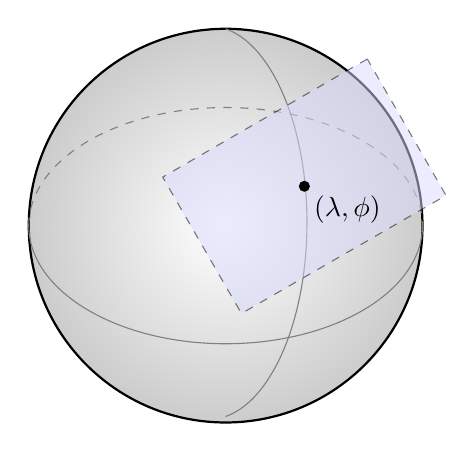
\begin{tikzpicture}[>=stealth]

    % 1. Define custom 3D projection vectors manually (Regular 2D coordinates)
    % This mimics a perspective view without the 3D library
    \coordinate (O) at (0,0);
    \def\R{2.5} % Radius of the sphere

    % 2. Draw the Sphere (Shading creates the 3D volume effect)
    \shade[inner color=white, outer color=gray!40] (O) circle (2.5);
    \draw[thick] (O) circle (\R);

    % 3. Draw Curvature Lines (Ellipses)
    % Equator-like curve
    \draw[gray, thin] (-\R,0) arc (180:360:{\R} and {0.6*\R});
    \draw[gray, dashed] (-\R,0) arc (180:0:{\R} and {0.6*\R});

    % Vertical curve (Longitude)
    \draw[gray, thin] (0,\R) arc (80:-80:{0.5*\R} and {\R});

    % 4. The Tangent Plane (A skewed quadrilateral)
    \coordinate (P) at (1, 0.5);
    \node [fill=blue!15, opacity=0.5, dashed, draw, shape=rectangle, minimum width=3cm, minimum height=2cm, anchor=center, rotate around={30:(P)}] at (P) {};

    % 5. Define the Target Point (P) on the surface
    \fill (P) circle (2pt) node[below right] {$(\lambda, \phi)$};

  \end{tikzpicture}

  \caption{Tangent space of $\S^2$}
  \label{fig:tangent_space_of_s2}
\end{figure}


A rather straightforward basis for the tangent space is given by
\[%
  \B = \left\{\left.\pdv{}{x^i}\right\rvert_a\right\}_{i=1}^{i=n}
,\]%
defined by
\[%
  \left.\pdv{}{x^i}\right\rvert_a f = \pdv{f}{x^i}(a)
.\]%

\begin{definition}
  A \emph{tangent bundle}, denoted as $TM$, of a manifold $M$ is defined as
  \[%
    TM = \bigsqcup_{p \in M} T_pM = \{(p, v) : p \in M, v \in T_pM\}
  .\]%
\end{definition}

\begin{figure}[h]
  \centering

  \begin{tikzpicture}[>=Stealth, scale=1.3]

    % --- 1. TOTAL SPACE TM (Top Left) ---
    \begin{scope}[shift={(-3.5,0)}]
      % Path definitions for the 3D "out-in-out" effect
      \def\Mcurve{(-2,0.2) to[out=20, in=160] (0,-0.1) to[out=-20, in=200] (2,0.2)}
      \def\TMtop{(-2,1) to[out=20, in=160] (0,0.7) to[out=-20, in=200] (2,1)}
      \def\TMbottom{(-2,-0.6) to[out=20, in=160] (0,-0.9) to[out=-20, in=200] (2,-0.6)}
      \def\TMpath{\TMtop -- (2,-0.6) -- \TMbottom -- (-2,-0.6) -- cycle}

      % Shading the local patch pi^-1(U)
      \begin{scope}
        \clip \TMpath;
        \fill[gray!30] (-1,-1.5) rectangle (1,1.5);

        % Vertical Fibers (Tangent Spaces T_pM)
        \foreach \x in {-1.9, -1.7, ..., 1.9} {
          \draw[gray!40, thin] (\x, -1.5) -- (\x, 1.5);
        }
      \end{scope}

      % Dashed boundaries for the patch
      \begin{scope}
        \clip \TMpath;
        \draw[thick, dashed] (-1,-1.5) -- (-1,1.5);
        \draw[thick, dashed] (1,-1.5) -- (1,1.5);
      \end{scope}

      % The Zero Section (s: M -> TM)
      \draw (-2, 0.2) to[out=20, in=160] (0, -0.1) to[out=-20, in=200] (2, 0.2);

      \draw[thick] \Mcurve;

      % Overlay thick line ONLY inside the patch area using clipping
      \begin{scope}
        \clip (-1,-1) rectangle (1,1);
        \draw[ultra thick] \Mcurve;
      \end{scope}

      \node[above] at (0, 1.1) {\large $TM$};
      \node[below] at (0.8, -1) {\large $\pi^{-1}(U)$};
    \end{scope}

    % --- 2. TARGET SPACE R^2n (Top Right) ---
    \begin{scope}[shift={(1.5,0)}]
      \filldraw[fill=gray!30, draw=white] (-1,-0.8) rectangle (1,0.8);

      \foreach \x in {-0.8, -0.6, ..., 0.8} {
        \draw[black, thin] (\x, -0.8) -- (\x, 0.8);
      }
      \draw[black, dashed] (-1, -0.8) -- (-1, 0.8);
      \draw[black, dashed] (1, -0.8) -- (1, 0.8);

      \draw[<->, ultra thick] (-1.8, 0) -- (1.8, 0);

      \node[above] at (0, 0.8) {\large $\mathbb{R}^{2n}$};
      \node[below] at (0, -0.8) {\large $\varphi(U) \times \mathbb{R}^n$};
    \end{scope}

    % --- 3. BASE MANIFOLD M (Bottom Left) ---
    \begin{scope}[shift={(-3.5,-3.5)}]
      % Define the curve base path to match TM bottom exactly
      \def\Mcurve{(-2,0.2) to[out=20, in=160] (0,-0.1) to[out=-20, in=200] (2,0.2)}

      % Draw regular thickness curve outside/inside
      \draw[thick] \Mcurve;

      % Overlay thick line ONLY inside the patch area using clipping
      \begin{scope}
        \clip (-1,-1) rectangle (1,1);
        \draw[ultra thick] \Mcurve;
      \end{scope}

      % Endpoint parentheses
      \node at (-0.98,0.2) {\huge (};
      \node at (0.98,-0.2) {\huge )};

      \node at (2.3, 0.3) {\large $M$};
      \node at (0, -0.4) {\large $U$};
    \end{scope}

    % --- 4. COORDINATE IMAGE phi(U) (Bottom Right) ---
    \begin{scope}[shift={(1.5,-3.5)}]
      \draw[<->, thick] (-1.8, 0.05) -- (1.8, 0.05);
      \draw[ultra thick] (-1, 0.05) -- (1, 0.05) node[midway, below] {\large $\phi(U)$};
      \draw[ultra thick] (-0.98, 0.05) node {\huge (} -- (0.98, 0.05) node {\huge )};
    \end{scope}

    % --- 5. MAPPING ARROWS ---
    \draw[->, thick, orange!80!black] (-1, 0.4) to[bend left=25] node[midway, above] {\huge $\widetilde{\varphi}$} (0.5, 0.4);
    \draw[->, thick, blue!70!black] (-2.8, -3.5) to[bend left=25] node[midway, above] {\huge $\varphi$} (1.3, -3.1);

    \draw[->, thick] (-3.5, -1.2) -- (-3.5, -2.8) node[midway, left] {\huge $\pi$};
    \draw[->, thick] (2, -1.2) -- (2, -2.8);

  \end{tikzpicture}

  \caption{Coordinates for the Tangent bundle}
  \label{fig:coordinates_for_the_tangent_bundle}
\end{figure}


\begin{definition}
  A \emph{vector bundle} over a manifold $M$ is a topological space $E$ together with a continuous surjection $\pi : E \to M$ such that for each point $p \in M$, the fiber $\pi^{-1}(p)$ is a vector space, and there exists an open neighborhood $U$ of $p$ in $M$ and a homeomorphism $\phi : \pi^{-1}(U) \to U \times \R^k$ that respects the vector space structure on the fibers.
\end{definition}

\begin{definition}
  A \emph{fibre} of a vector bundle $E$ over a manifold $M$ at a point $p \in M$ is the vector space $\pi^{-1}(p)$, where $\pi : E \to M$ is the projection map of the vector bundle.
\end{definition}

\begin{definition}
  A \emph{cotangent bundle} of a manifold $M$ is the vector bundle $T^*M$ whose fiber at each point $p \in M$ is the cotangent space at $p$, denoted by $T_p^*M$. The elements of $T_p^*M$ are called \emph{covariant vectors} or simply \emph{covectors}.
\end{definition}

\begin{note}
  Covectors live in the cotangent bundle, while the contravariant vectors (i.e., tangent vectors) live in the tangent bundle.
\end{note}

In local coordinates, tensor components are written using upper and lower indices to distinguish components with respect to a chosen basis of $T_pM$ and its dual basis in $T_p^*M$.

\begin{definition}
  Let $\pi : E \to M$ be a vector bundle over $M$. A \emph{section} of $E$ is a smooth map
  \[%
    s : M \to E
  ,\]%
  such that
  \[%
    \pi \circ s = \mathrm{id}_M
  .\]%
  The space of smooth sections of $E$ is denoted $\Gamma(E)$.
\end{definition}

\begin{figure}[h]
  \centering

  \begin{tikzpicture}[>=Stealth, scale=1.2]

    % --- BASE MANIFOLD M (Bottom) ---
    \begin{scope}[shift={(0,-3.5)}]
      % Base Manifold M
      \draw[thick] plot [smooth cycle, tension=0.7] coordinates {(-2.5,0) (-1,0.5) (1.5,0.3) (2.5,-0.2) (1,-0.6) (-1.5,-0.5)};
      \node at (2.8, 0) {$M$};

      % Subset U with parentheses
      \draw[ultra thick] (-1.3, -0.1) to[out=10, in=170] (1.3, -0.1);
      \node at (-1.4, -0.1) {\large (};
      \node at (1.4, -0.1) {\large )};
      \node at (0, -0.4) {$U$};
    \end{scope}

    % --- TOTAL SPACE REGION pi^-1(U) (Top Left) ---
    \begin{scope}[shift={(-3,0)}]
      % The curvy bundle volume
      \filldraw[fill=gray!20, draw=black]
        (-1.5,0) to[out=10, in=190] (1.5,0) -- (1.5,1.5)
        to[out=190, in=10] (-1.5,1.5) -- cycle;

      % Wavy top face
      \filldraw[fill=gray!40, draw=black]
        (-1.5,1.5) to[out=10, in=190] (0.5,1.8) to[out=10, in=170] (1.5,1.5)
        to[out=210, in=-10] (-0.5,1.2) to[out=170, in=-10] (-1.5,1.5);

      % Vertical Fibers
      \foreach \x in {-1.2, -0.9, -0.6, -0.3, 0, 0.3, 0.6, 0.9, 1.2} {
        \draw[gray!60, thin] (\x, 0.05) -- (\x, 1.45);
      }

      % Dashed boundary lines
      \draw[dashed] (-0.7,0) -- (-0.7,1.3);
      \draw[dashed] (0.8,0) -- (0.8,1.4);

      % Highlighted Section
      \draw[ultra thick] (-1.1, 0.5) to[out=10, in=190] (1.4, 0.7);

      \node at (1.8, 1.8) {$E$};
      \node at (0, -0.3) {$\pi^{-1}(U)$};
    \end{scope}

    % --- TRIVIAL PRODUCT U x R^k (Top Right) ---
    \begin{scope}[shift={(3,0)}]
      % Rectangle volume
      \filldraw[fill=gray!20, draw=black] (-1.5,0) rectangle (1.5,1.5);

      % Vertical Fibers
      \foreach \x in {-1.2, -0.9, -0.6, -0.3, 0, 0.3, 0.6, 0.9, 1.2} {
        \draw[gray!60, thin] (\x, 0) -- (\x, 1.5);
      }

      % Highlighted Section (Straight)
      \draw[ultra thick] (-1.5, 0.6) -- (1.5, 0.6);

      \node at (2.2, 0.75) {$U \times \mathbb{R}^k$};
    \end{scope}

    % --- MAPPING ARROWS ---

    % Trivialization Map Phi
    \draw[->, thick] (-1.2, 0.75) to[out=20, in=160] node[midway, above] {$\Phi$} (1.2, 0.75);

    % Projection Map from E
    \draw[->, thick] (-1.5, -0.5) -- (-0.5, -1.8) node[midway, left] {$p$};

    % Projection Map from U x R^k
    \draw[->, thick] (1.5, -0.5) -- (0.5, -1.8) node[midway, right] {$p$};

  \end{tikzpicture}

  \caption{Fibres and Sections}
  \label{fig:fibres_and_sections}
\end{figure}


Now, with all that out of the way, we can finally define a tensor.

\begin{definition}
  Let $M$ be a manifold and $p \in M$. An \emph{$(r,s)$-tensor at $p$} is a multilinear map
  \[%
    T_p : (T_p^*M)^r \times (T_pM)^s \to \R
  .\]%
  An \emph{$(r,s)$-tensor field} on $M$ is a smooth section of the tensor bundle
  \[%
    (T^*M)^{\otimes r} \otimes (TM)^{\otimes s}
  .\]%
\end{definition}

\subsection{Differentials of Maps} We now define the differential of a map between two manifolds.
\begin{definition}
  Let $F : M \to N$ be a smooth map between two manifolds $M$ and $N$. For each point $p \in M$, we define the \emph{differential of $F$ at $p$} by
  \[%
    \dF_p : T_pM \to T_{F(p)}N
  .\]%
\end{definition}

\begin{figure}[ht]
  \centering
  \begin{tikzpicture}[>=Stealth, scale=1.2]

    % --- MANIFOLD M ---
    \filldraw[fill=green!10, draw=green!40!black, thick]
      plot [smooth cycle, tension=0.7] coordinates {(-2,0.5) (0,1.5) (2,1) (3,-0.5) (1,-1.5) (-2,-1)};
    \node at (2.2, -0.8) {\large $M$};

    \draw[thick] (1.4,0.1) to[out=-40, in=220] (2.4,0.1);
    \draw[thick] (1.5,0) to[out=40, in=140] (2.3,0);

    % Tangent Plane T_pM
    \coordinate (p) at (-0.8, 0.4);
    \begin{scope}[shift={(p)}]
      % Tangent plane parallelogram
      \filldraw[fill=gray!20, draw=gray!60, thick, fill opacity=0.7]
        (-1.2,-0.4) -- (1.6,-0.4) -- (2.4,1.4) -- (-0.4,1.4) -- cycle;
      \node at (1.9, 1.2) {\large $T_pM$};

      % Vector v starting from a point on the plane
      \coordinate (v_base) at (0.3, 0.3);
      \fill (v_base) circle (1.5pt) node[left] {\large $v$};
      \draw[->, thick] (v_base) -- +(0.4, 0.7) node[right] {\large $v$};
    \end{scope}
    \fill (p) circle (2pt) node[below left] {\large $p$};

    % --- MANIFOLD N ---
    \begin{scope}[shift={(5,0)}]
      \filldraw[fill=blue!5, draw=blue!40!black, thick]
        plot [smooth cycle, tension=0.8] coordinates {(0,2.2) (2.5,1.5) (3,-1) (1,-1.8) (-0.5,-0.5)};
      \node at (2.5, -0.8) {\large $N$};

      % Tangent Plane T_F(p)N
      \coordinate (Fp) at (0.4, 0.3);
      \begin{scope}[shift={(Fp)}]
        \filldraw[fill=gray!20, draw=gray!60, thick, fill opacity=0.7]
          (-1.5,-1.2) -- (1.4,-0.4) -- (1.7,1.8) -- (-1.2,1.0) -- cycle;
        \draw[fill=gray!20, draw=gray!60, thick, fill opacity=0.7] (-1.5,-1.2) -- (-1.2,1.0) node[below right, xshift=5, yshift=2] {\large $T_{F(p)}N$};

        % Pushed forward vector dF_p(v)
        \coordinate (dfv_base) at (0,0);
        \fill (dfv_base) circle (1.5pt) node[below left] {\large $F(p)$};
        \draw[->, thick] (dfv_base) -- (1, 0.7) node[above] {\large $dF_p(v)$};
      \end{scope}
    \end{scope}

    \begin{scope}[shift={(0,-4)}]
      \draw[<->, thick] (0,-2) -- (0,2) node[right] {\large $\R$};
      \draw (-0.2, 0) -- (0.2, 0);
    \end{scope}

    % --- MAP f and REAL LINE R ---
    \draw[->, thick] (0.3, -3) to[bend right=25] node[above] {\large $f$} (6, -2);
    % --- MAPPING ARROW F ---
    \draw[->, thick] (2.5, 0.8) to[bend left=25] node[above] {\large $F$} (4, 0.8);

  \end{tikzpicture}
  \caption{The differential}
\end{figure}


\subsection{Differential Forms and the Wedge Product} Next, we introduce the concept of a differential form. A very well-known example of a differential form is $\dx$, which is a 1-form. Formally, we can define a 1-form as follows.

\begin{definition}
  A \emph{1-form} on a manifold $M$ is a smooth section of the cotangent bundle $T^*M$, that is,
  \[%
    \omega \in \Gamma(T^*M)
  ,\]%
  where $\omega : M \to T^*M$ is a smooth map such that $\pi \circ \omega = \mathrm{id}_M$. Equivalently, for each $p \in M$, a 1-form assigns a covector $\omega_p \in T_p^*M$ smoothly in $p$.
\end{definition}

A 1-form represents a linear functional that takes a tangent vector at a point and produces scalar.

\begin{example}
  In local coordinates $\{x^\mu\}$, a 1-form $\omega$ can be written as
  \[%
    \omega = \omega_\mu \dx^\mu
  .\]%
  If $v = v^\mu \pd{\mu} \in T_pM$, then
  \[%
    \omega(v) = \omega_\mu v^\mu
  .\]%
\end{example}

We denote the space of smooth 1-forms on $M$ by $\Omega^k(M)$, with $k = 1$. This implies that there are higher order forms. So, we need a way to generalize this to higher-order forms, which is where the concept of the wedge product comes in. The wedge product allows us to combine 1-forms to create higher-order forms, such as 2-forms, 3-forms, etc. We can define the wedge product as follows.

\begin{definition}
  The \emph{wedge product}
  \[%
    \wedge : \Omega^p(M) \times \Omega^q(M) \to \Omega^{p+q}(M)
  ,\]%
  is the bilinear operation that takes a $p$-form $\alpha$ and a $q$-form $\beta$ and produces a $(p+q)$-form $\alpha \wedge \beta$, defined by the following properties:
  \begin{enumerate}
    \item \emph{Bilinearity:} For all $\alpha, \alpha' \in \Omega^p(M)$, $\beta, \beta' \in \Omega^q(M)$, and $f, g \in C^\infty(M)$,
      \begin{align*}
        (f\alpha + g\alpha') \wedge \beta &= f(\alpha \wedge \beta) + g(\alpha' \wedge \beta), \\
        \alpha \wedge (f\beta + g\beta') &= f(\alpha \wedge \beta) + g(\alpha \wedge \beta').
      \end{align*}
    \item \emph{Antisymmetry:} For all $\alpha \in \Omega^p(M)$ and $\beta \in \Omega^q(M)$,
      \[%
        \alpha \wedge \beta = (-1)^{pq} \beta \wedge \alpha
      .\]%
      In particular, if $\alpha$ is a 1-form, then $\alpha \wedge \alpha = 0$.
    \item \emph{Associativity:} For all $\alpha \in \Omega^p(M)$, $\beta \in \Omega^q(M)$, and $\gamma \in \Omega^r(M)$,
      \[%
        (\alpha \wedge \beta) \wedge \gamma = \alpha \wedge (\beta \wedge \gamma)
      .\]%
  \end{enumerate}
\end{definition}

Now, we can use the wedge product to define a 2-form, which represents an orientated area element on the manifold. Just like in vector calculus, where we had $\dA = \dx\dy$, we can define a 2-form $\omega$ as
\[%
  \omega = \omega_{\mu\nu} \dx^\mu \wedge \dx^\nu
.\]%

Next, we need to define what the pullback of a differential form is and what a pushforward of a vector field is. The pullback allows us to take a differential form defined on one manifold and pull it back to another manifold via a smooth map, while the pushforward allows us to take a vector field defined on one manifold and push it forward to another manifold via a smooth map.

\begin{definition}
  Let $f : M \to N$ be a smooth map between manifolds $M$ and $N$. The \emph{pullback} of a differential form $\omega$ on $N$ by the map $f$ is a differential form on $M$, denoted by $f^*\omega$, defined as follows: for any point $p \in M$ and any tangent vectors $v_1, v_2, \ldots, v_k \in T_pM$, we have
  \[%
    (f^*\omega)_p(v_1, v_2, \ldots, v_k) = \omega_{f(p)}(\df_p(v_1), \df_p(v_2), \ldots, \df_p(v_k))
  .\]%
\end{definition}

\begin{example}
  Let $F : \R^2 \setminus \{0\} \to \R^2$ be defined by the polar coordinate transformation
  \[%
    F(r,\theta) = (x,y) = (r\cos\theta, r\sin\theta)
  .\]%
  We compute the pullback of the coordinate $1$-forms $\dx$ and $\dy$.

  Since
  \[%
    x = r\cos\theta \quad \aand y = r\sin\theta
  ,\]%
  we have
  \[%
    \dx = \cos\theta \dr - r\sin\theta \dd{\theta} \aand \dy = \sin\theta \dr + r\cos\theta \dd{\theta}
  .\]%
  Therefore,
  \[%
    F^*(\dx) = \cos\theta \dr - r\sin\theta \dd{\theta} \aand F^*(\dy) = \sin\theta \dr + r\cos\theta \dd{\theta}
  .\]%
  As an application, consider the standard area form $\dx \wedge \dy$. Using the bilinearity and antisymmetry of the wedge product, we compute
  \begin{align*}
    F^*(\dx \wedge \dy) &= F^*(\dx) \wedge F^*(\dy) \\
                      &= (\cos\theta \dr - r\sin\theta \dd{\theta}) \wedge (\sin\theta \dr + r\cos\theta \dd{\theta}) \\
                      &= r \dr \wedge \dd{\theta}.
  \end{align*}
  Thus, the pullback naturally produces the Jacobian factor $r$ appearing in polar coordinates.
\end{example}

When we're computing pullbacks of differential forms, we can use the formula
\[%
  f^*\left(\bigwedge_{i=1}^k \du^i\right) = \bigwedge_{i=1}^k f^*(\du^i) = \bigwedge_{i=1}^k \pd{j} u^i \dx^j
.\]%

\begin{definition}
  Let $f : M \to N$ be a smooth map between manifolds $M$ and $N$. The \emph{pushforward} of a vector field $X$ on $M$ by the map $f$ is a vector field on $N$, denoted by $f_*X$, defined as follows: for any point $p \in M$, we have
  \[%
    (f_*X)_{f(p)} = \df_p(X_p)
  .\]%
\end{definition}

\begin{example}
  Let $F : \R^2 \to \R^2$ be defined by
  \[%
    F(x,y) = (u,v) = (x^2 - y, x + y)
  .\]%
  We compute the pushforward of the vector field $X = \pd{x}$.

  The Jacobian matrix of $F$ is
  \[%
    \dF = \begin{pmatrix}
      \pd{x} u & \pd{y} u \\
      \pd{x} v & \pd{y} v \\
    \end{pmatrix}
    = \begin{pmatrix}
      2x & -1 \\
      1 & 1 \\
    \end{pmatrix}
  .\]%
  Since $\pd{x}$ corresponds to the vector $(1,0)$ in coordinates, we obtain
  \[%
    F_*(\pd{x}) = 2x \pd{u} + \pd{v}
  .\]%
  Thus, the pushforward transforms the coordinate basis vector $\pd{x}$ into a linear combination of the coordinate basis vectors $\pd{u}$ and $\pd{v}$.
\end{example}

\begin{figure}[h]
  \centering

  \begin{tikzpicture}[>=Stealth, scale=1.2]

    % --- MANIFOLD M (Left Green) ---
    \begin{scope}
      \filldraw[fill=green!20, draw=green!40!black, thick]
        plot [smooth cycle, tension=0.7] coordinates {(-3,0) (-1,1.5) (1,0.5) (0.5,-1.5) (-2,-1)};
      \node at (0.5, -0.5) {$M$};
    \end{scope}

    % --- MANIFOLD N (Right Green) ---
    \begin{scope}[shift={(4,0)}]
      \filldraw[fill=green!20, draw=green!40!black, thick]
        plot [smooth cycle, tension=0.7] coordinates {(-1,0) (1,1.5) (3,0.5) (2.5,-1.5) (0,-1)};
      \node at (0, -0.5) {$N$};
    \end{scope}

    % --- MAPPINGS ---
    % phi
    \draw[->, thick] (1.2, 0.2) to[out=25, in=155] node[midway, above] {$\phi$} (3, 0.2);
    % T_p phi
    \draw[->, thick] (-0.2, 1.8) to[out=30, in=150] node[midway, above] {$T_p \phi$} (5.5, 1.7);

    % --- TANGENT PLANE M ---
    \coordinate (phiP) at (6.5, 1.2);
    \begin{scope}[shift={(4.3,-0.8)}]
      \filldraw[fill=blue!30, opacity=0.7, draw=blue!50!black, thick]
        (-1,1.3) -- (1.5,2.5) -- (2.5,1.5) -- (0,0.3) -- cycle;
      \node at (1.8, 2.7) {$T_{\phi(p)}N$};
      \fill (0.5, 1.2) circle (1.5pt) node[above right] {\tiny $\phi(p)$};
      \draw[->, brown!70!black, very thick] (0.5, 1.2) -- (-0.5, 1.4) node[above right, xshift=3.5, yshift=-2] {\tiny $T_p\phi \cdot v_p$};
      % Transformed curve
      \draw[blue!60!black, thick] (-0.5,1) to[out=20, in=180] (0.5,1.2) to[out=0, in=150] (2,0.8);
      \node[xshift=-7.5, yshift=3] at (0.5, 0.7) {\tiny $[\phi \circ \gamma]_{\phi(p)}$};
    \end{scope}

    % --- TANGENT PLANE N ---
    \coordinate (P) at (-1, 0.2);
    \begin{scope}[shift={(0,-1)}]
      \filldraw[fill=blue!30, opacity=0.7, draw=blue!50!black, thick]
        (-2.5,1.5) -- (-0.5,2.8) -- (0.5,0.8) -- (-1.5,-0.5) -- cycle;
      \node at (-2.3, 2.7) {$T_pM$};
      \fill (P) circle (1.5pt) node[left] {$p$};
      \draw[->, red!70!black, very thick] (P) -- (0, 1.7) node[above left] {$v_p$};
      % Curve gamma
      \draw[blue!60!black, thick] (-1.5,0.5) to[out=40, in=220] (P) to[out=40, in=200] (0.2,1.3);
      \node at (-1, 0.5) {$[\gamma]_p$};
    \end{scope}

    % --- INTERVAL AT BOTTOM LEFT ---
    \begin{scope}[shift={(0,0.5)}]
      \draw[thick] (-3,-3.5) -- (-0,-3.5);
      \draw[ultra thick, blue!40!black] (-2.2,-3.5) -- (-0.8,-3.5);

      % Opening parenthesis "(" at -epsilon
      \draw[thick] (-2.15, -3.3) arc (150:210:0.4);
      % Closing parenthesis ")" at epsilon
      \draw[thick] (-0.85, -3.7) arc (-30:30:0.4);

      \draw (-2.2, -3.7) node[below] {$-\varepsilon$};
      \draw (-0.8, -3.7) node[below] {$\varepsilon$};
      \draw (-1.5, -3.4) -- (-1.5, -3.6) node[below] {$0$};
      \draw[->] (-1.5, -3.3) to[bend left] node[midway, left] {$\gamma$} (-1.6,-1.1);
    \end{scope}

    % --- COTANGENT SPACES (Upper Part) ---
    \begin{scope}[shift={(0,4)}]
      \filldraw[fill=red!10, draw=red!60!black, thick] (-2, -1) rectangle (0.5, 1);
      \node at (-1.5, 1.2) {$T^*_p M$};
      \fill (-1, 0) circle (1.5pt) node[below] {$p$};
      \draw[->, thick] (-1, 0) -- (-1.5, 0.6) node[right] {$T^*_p \phi \cdot \alpha_{\phi(p)}$};

      \filldraw[fill=red!10, draw=red!60!black, thick] (4, -1) rectangle (6.5, 1);
      \node at (4.5, 1.2) {$T^*_{\phi(p)} N$};
      \fill (5, 0) circle (1.5pt) node[below] {$\phi(p)$};
      \draw[->, thick] (5, 0) -- (5.6, 0.5) node[above] {$\alpha_{\phi(p)}$};

      \draw[<-, thick] (0.7, 0.5) to[out=20, in=160] node[midway, above] {$T^*_p \phi$} (3.8, 0.5);
    \end{scope}

  \end{tikzpicture}

  \caption{Pushforward and pullback under a smooth map $\phi : M \to N$.}
  \label{fig:pushforward_and_pullback}
\end{figure}


\subsection{Curvature} Next, we introduce the concept of curvature on a manifold. In order to describe curvature on a manifold, we must first introduce the notion of a connection, which allows us to differentiate vector fields in a manner compatible with the smooth structure of the manifold.

\begin{definition}
  A \emph{connection} (or \emph{covariant derivative}) on a manifold $M$ is a map
  \[%
    \nabla : \Gamma(TM) \times \Gamma(TM) \to \Gamma(TM)
  ,\]%
  denoted $(X,Y) \mapsto \nabla_X Y$, satisfying the following properties for all vector fields $X,Y,Z \in \Gamma(TM)$ and smooth functions $f \in C^\infty(M)$:
  \begin{enumerate}
    \item $\nabla_{fX + Z} Y = f \nabla_X Y + \nabla_Z Y$,
    \item $\nabla_X (Y + Z) = \nabla_X Y + \nabla_X Z$,
    \item $\nabla_X (fY) = X(f) Y + f \nabla_X Y$.
  \end{enumerate}
\end{definition}

The connection measures how a vector field changes in the direction of another vector field. Unlike ordinary differentiation in Euclidean space, this notion does not require an ambient space.

In local coordinates $\{x^\mu\}$, a connection is determined by its Christoffel symbols $\Gamma^\rho_{\mu\nu}$, defined by
\[%
  \nabla_{\pd{\mu}} \pd{\mu} = \Gamma^\rho_{\mu\nu} \pd{\rho}
.\]%
For a vector field $V = V^\nu \pd{\nu}$, the covariant derivative is given by
\[%
  \nabla_\mu V^\rho = \pd{\mu} V^\rho + \Gamma^\rho_{\mu\nu} V^\nu
.\]%

Associated to any connection is its torsion tensor.

\begin{definition}
  The \emph{torsion tensor} $T$ of a connection $\nabla$ is defined by
  \[%
    T(X,Y) = \nabla_X Y - \nabla_Y X - [X,Y]
  ,\]%
  where $[X,Y]$ denotes the Lie bracket of vector fields. A connection is said to be \emph{torsion-free} if $T = 0$.
\end{definition}

We now define curvature.
\begin{definition}
  The \emph{Riemann curvature tensor} associated to a connection $\nabla$ is the $(1,3)$-tensor defined by
  \[%
    R(X,Y)Z = \nabla_X \nabla_Y Z - \nabla_Y \nabla_X Z - \nabla_{[X,Y]} Z
  .\]%
\end{definition}

The curvature tensor measures the failure of second covariant derivatives to commute.

In local coordinates, its components are given by
\[%
  R^\rho_{\sigma\mu\nu} = \pd{\mu} \Gamma^\rho_{\nu\sigma} - \pd{\mu} \Gamma^\rho_{\mu\sigma} + \Gamma^\rho_{\mu\lambda} \Gamma^\lambda_{\nu\sigma} - \Gamma^\rho_{\nu\lambda} \Gamma^\lambda_{\mu\sigma}
.\]%

The Riemann tensor satisfies several important symmetry properties. In particular,
\[%
  R^\rho_{\sigma\mu\nu} = - R^\rho_{\sigma\nu\mu}
.\]%

If the connection is torsion-free and compatible with a metric (to be introduced later), additional symmetries arise.

From the Riemann tensor we obtain contractions.
\begin{definition}
  The \emph{Ricci tensor} is defined by the contraction
  \[%
    R_{\sigma\nu} = R^\rho_{\sigma\rho\nu}
  .\]%
\end{definition}

If a metric $g_{\mu\nu}$ is given, we may further contract to obtain the scalar curvature.

\begin{definition}
  The \emph{scalar curvature} is defined by
  \[%
    R = g^{\sigma\nu} R_{\sigma\nu}
  \]%
\end{definition}

\subsection{Parallel Transport and Geodesics} Let $(M, g)$ be a manifold equipped with a Levi-Civita connection $\nabla$.

Let $\gamma : I \to M$ be a smooth curve, where $I \subset \R$ is an interval. Denote its tangent vector by
\[%
  \dot{\gamma}(t) = \odv{\gamma}{t}
.\]%

If $X$ is a vector field defined along $\gamma$, meaning
\[%
  X(t) \in T_{\gamma(t)} M
,\]%
then the \emph{covariant derivative of $X$ along $\gamma$} is defined by
\[%
  \codv{X}{t} := \nabla_{\dot{\gamma}(t)} X
.\]%

This measures how $X$ changes along the curve while accounting for the curvature of the manifold.

In local coordinates $\{x^\mu\}$, if
\[%
  X = X^\mu \pd{\mu}
,\]%
then
\[%
  \codv{X^\mu}{t} = \odv{x^\mu}{t} + \Gamma^\mu_{\alpha\beta} \dot{\gamma}^\alpha X^\beta
.\]%
A vector field $X$ along $\gamma$ is said to be \emph{parallel transported} if
\[%
  \codv{\dot{\gamma}}{t} = 0
.\]%
In coordinates, this becomes
\[%
  \odv{X^\mu}{t}
  +
  \Gamma^\mu_{\alpha\beta}
  \dot{\gamma}^\alpha
  X^\beta
  =
  0.
\]%
Thus parallel transport preserves the vector with respect to the connection.

If $\nabla$ is metric-compatible (as for the Levi-Civita connection), parallel transport preserves inner products:
\[%
  \odv{}{t} g(X, Y) = 0
,\]%
whenever $X$ and $Y$ are parallel along $\gamma$.

A curve $\gamma$ is called a \emph{geodesic} if its tangent vector is parallel transported along itself:
\[%
  \codv{\dot{y}}{t} = 0
.\]%
Equivalently,
\[%
  \nabla_{\dot{\gamma}} \dot{\gamma} = 0
.\]%
In local coordinates, this yields the geodesic equation:
\[%
  \odv[2]{x^\mu}{t} + \Gamma^\mu_{\alpha\beta} \odv{x^\alpha}{t} \odv{x^\beta}{t} = 0
.\]%

Thus geodesics are curves whose acceleration vanishes with respect to the connection.

If $(M, g)$ is pseudo-Riemannian, geodesics can also be characterized as stationary points of the energy functional
\[%
  E[\gamma] = \frac{1}{2} \int g_{\mu\nu} \dot{x}^\mu \dot{x}^\nu \dt
.\]%

Applying the Euler–Lagrange equations to this functional yields precisely the coordinate geodesic equation above.

The quantitative description of this relative acceleration is given by the geodesic deviation equation, which will be discussed later.
